% Einleitung
\section{Einleitung}

Ziel des Projektes ist die Entwicklung einer Web-basierten Nutzerschnittstelle zur Visualisierung von Luftqualitätsdaten.
Die Qualität der Luft ist essentiell für die Gesundheit und Lebensqualität der Menschen. So kann beispielsweise eine zu hohe Konzentration von Feinstaub langfristig die Lunge schädigen. 
In den letzten Jahren haben Schadstoffwerte in der Luft an Bedeutung gewonnen.
Durch ein heterogenes Netzwerk von \glspl{Sensor} werden deutschlandweit Luftqualitätsdaten erfasst und in Datenbanken gespeichert.
Viele bereits existierende Plattformen zur Visualisierung dieser Daten sind an professionelle Nutzer gerichtet. Somit sind diese Anwendungen wenig für die Nutzung durch die breite Masse geeignet.
\\
Die Besonderheit dieser Datensammlung besteht auch darin, dass sich die Typen der Sensoren stark unterscheiden. Sowohl diverse \gls{DIY}-\glspl{Sensor} von privaten Teilnehmern, als auch professionelle Messstationen tragen ihre Werte in die Datenbank ein. 
\\
\begin{figure}[h]
    \centering
    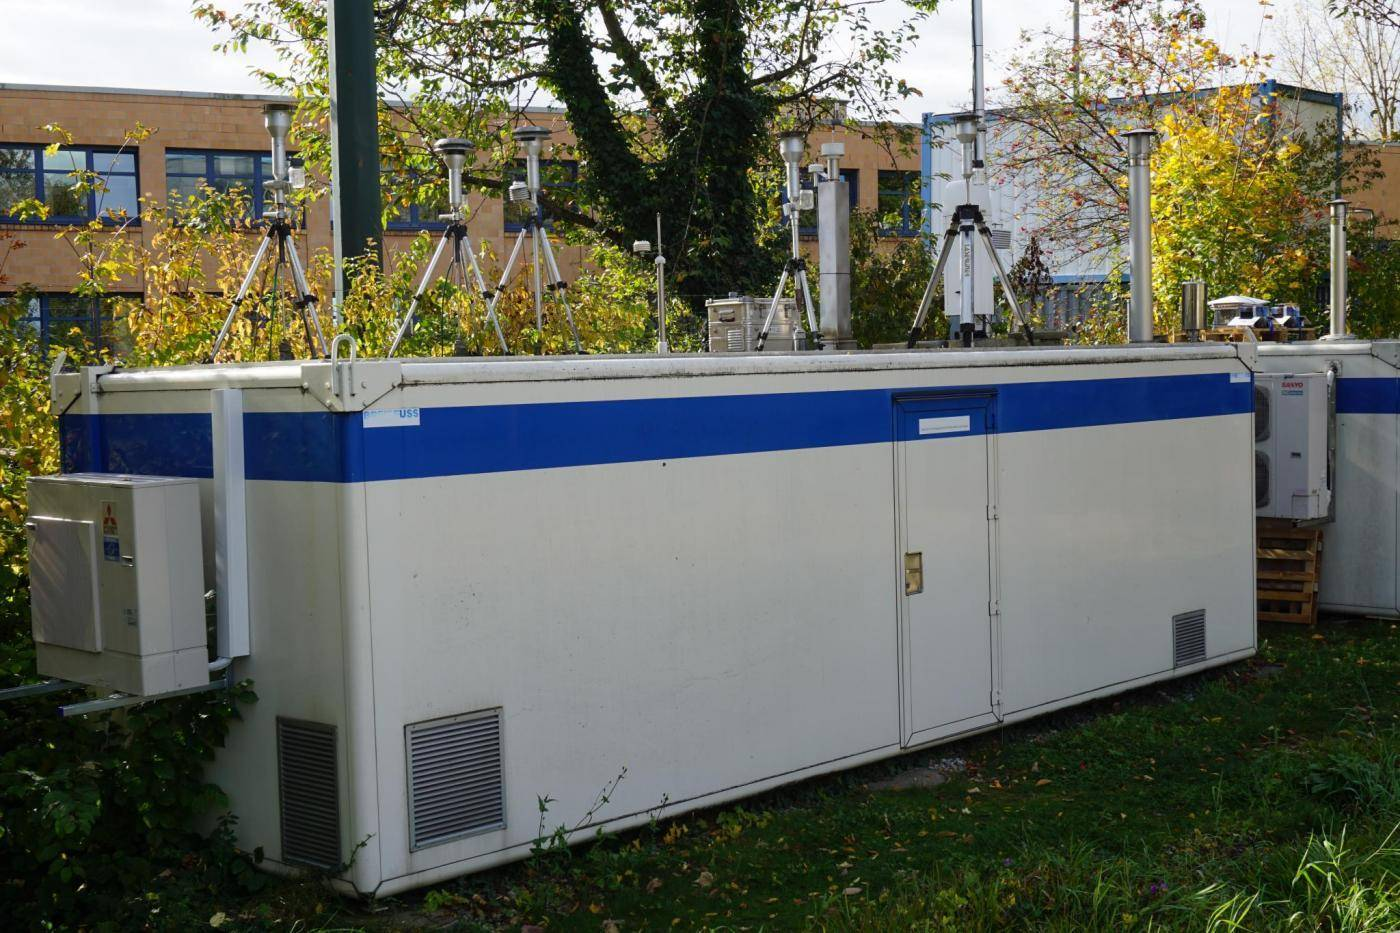
\includegraphics[scale=0.25] {media/Sensor.JPG}
    \caption{Professionelle Messstationen zur Erhebung von \gls{Luftqualitaetsdaten} (Quelle: https://www.smartaq.net/de/gallery/)}
\end{figure}
In den Datenbanken werden verschiedene Parameter der Luftqualität erfasst. Beispiele für mögliche Messwerte sind:
\begin{itemize} [noitemsep]
    \item \gls{Feinstaub}konzentration
    \item Lufttemperatur
    \item Luftfeuchtigkeit
    \item Luftdruck
\end{itemize}
Durch diese Anwendung können die Daten aus diversen Messstationen einer großen Gruppe von Nutzern anschaulich zugänglich gemacht werden.\\
Probieren Sie \softwarename aus und überzeugen Sie sich selbst!